\documentclass[11pt]{report}

\usepackage[toc,page]{appendix}
\usepackage{amsmath}
\usepackage{stmaryrd}
\usepackage{syntax}
\usepackage{tikz}
% Chapter number and name on one line
\usepackage{titlesec}
\titleformat{\chapter}[hang] 
{\normalfont\huge\bfseries}{\thechapter}{1em}{} 
% No new page after chapter
\usepackage{etoolbox}
\makeatletter
\patchcmd{\chapter}{\if@openright\cleardoublepage\else\clearpage\fi}{}{}{}
\makeatother

\usetikzlibrary{shapes,arrows}
\tikzstyle{internalStage} = [rectangle, draw, fill=blue!20, 
    text width=5em, text centered, minimum height=4em]
\tikzstyle{conversion} = [draw, -latex']

\title{LJSP - A LISP to asm.js compiler}
\author{Jan S\"ondermann}
\date{1st January 1900}

\newcommand{\eqdef}{\stackrel{\text{def}}{=}}%
\newcommand{\cpstrans}[1]{\ensuremath{\mathcal{K}\llbracket #1 \rrbracket}}

\begin{document}
% TODO
% why scala? why LLVM IR/C



\maketitle

\begin{center}
\textbf{Originality avowal}
\end{center}

I verify that I am the sole author of this report, except where explicitly stated to the contrary.

I grant the right to King's College London to make paper and electronic copies of the submitted work for purposes of marking, plagiarism detection and archival, and to upload a copy of the work to Turnitin or another trusted plagiarism detection service.

\begin{flushright}
Jan Söndermann \\
@@date@@@
\end{flushright}
\newpage
			
\begin{center}
\textbf{Abstract}
\end{center}

@@@
\newpage

\begin{center}
\textbf{Acknowledgements}
\end{center}
I would like to thank my supervisor Dr. Christian Urban for supervising my project and for providing me with both guidance and freedom.
\newpage

\tableofcontents

\chapter{Introduction}
One of the main trends of today's Internet is the shift from traditionally offline or standalone programs to the web. This phenomenon, often @dubbed@ "Web 2.0"@ajax@ is visible in the success of web applications such as GMail and Facebook @other examples@.

This success of the web has brought with it the rise of the programming language it is build on: JavaScript, the only language that is supported by all major browsers. Statistics, such as the number of repositories created on GitHub (a popular code sharing website) using JavaScript, show this success: in 2013, JavaScript led this list by a substantial margin. @cite

Since JavaScript is no longer confined to being used for simple animation and input-validation tasks, the complexity of web apps has increased tremendously. Modern JavaScript frameworks, such as Ember.js@link or Meteor@link use the full register of functionality the language offers and are @just as complex as traditional web frameworks that use languages such as Ruby or Python.@

Unfortunately, this proliferation of JavaScript has taken the language far beyond the tasks it was initially conceived for @cite. There is a widespread consensus@cite the language has a number of shortcomings. Brendan Eich, the creator of JavaScript, writes about its early history:
\begin{quote}
In April 1995 I joined Netscape in order to "add Scheme to the browser." [...]

So in 10 days in May 1995, I prototyped "Mocha," the code name Marc Andreessen had chosen. [...]

To overcome all doubts, I needed a demo in 10 days. I worked day and night, and consequently made a few language-design mistakes (some recapitulating bad design paths in the evolution of LISP), but I met the deadline and did the demo.
\end{quote}
% http://chimera.labs.oreilly.com/books/1234000001808/pr02.html

Criticism of JavaScript has mostly focussed on two areas:
\begin{itemize}
\item Inconsistencies and mistakes in the design of the language. Examples for this often given include the confusion around JavaScript's large number of falsy values (\texttt{0},  \texttt{''}, \texttt{NaN}, \texttt{false}, \texttt{null} and \texttt{undefined}) and its set of reserved keywords, which includes a large number of words not in use by the language but doesn't include \texttt{NaN} and \texttt{undefined}. This makes it necessary to test for \texttt{undefined}ness using \\
\mbox{\texttt{typeof x === 'undefined'}} to avoid comparing against a redefined \texttt{undefined}.
\item Slow execution speed. Writing fast interpreters for JavaScript has been an extraordinary difficult task for browser @manufacturers. @why?@
\end{itemize}

Programmers have responded to the first problem in ways that include limiting themselves to a subset of JavaScript that excludes the inconsistent and badly-designed parts (cf. the very popular "JavaScript: The Good Parts"@cite). Another response has been to create new languages that compile to JavaScript, such as the very popular CoffeeScript @cite, Microsoft's TypeScript and Google's Dart.

The second problem has been partly remedied by a new generation of JavaScript engines spearheaded by Google's V8, released in 2008 as part of Google Chrome. The other browser makers, including Mozilla soon followed by rewriting their own JavaScript engines. These new engines often brought impressive speed gains.

In early 2013, Mozilla released asm.js, a project that claims to take these two approaches to their logical conclusion. It defines an extremely limited, statically typed subset of JavaScript that can be executed very quickly. This subset is intended as compilation targets for high level languages.

This project defines such a language and provides a compiler for it that outputs, among other targets, asm.js. It sets out to explore the performance @@

\chapter{Background \& Existing Work}
\section{Technologies involved}
\subsection{asm.js}
\subsection{emscripten and LLVM}
\section{Similar Languages}

\chapter{Requirements}
\section{User Requirements}
\section{System Requirement}

\chapter{Specification}
\section{LJSP Grammar}
The grammar of LJSP in Extended Backus-Naur Form is given below.
\begin{grammar}
<program> ::= <defines> [ <expr> ] <defines>

<defines> ::= <define> <defines> | $\epsilon$

<define> ::= `(define (' <ident> <params> `)' <expr> `)'

<expr> ::= <double>
\alt <ident>
\alt `(if' <expr> <expr> <expr> `)'
\alt <lambda>
\alt `(let (' <letblocks> `)' <expr> `)'
\alt `(' <primOp> <args> `)'
\alt `(' <expr> <args> `)'

% add scientific form
<double> ::= \texttt{-?(\textbackslash d+(\textbackslash.\textbackslash d*)?|\textbackslash d*\textbackslash.\textbackslash d+)}

<ident> ::= \texttt{[a-zA-Z=*+/\textless\textgreater!?-][a-zA-Z0-9=*+/\textless\textgreater!?-_]*}

<lambda> ::= `(lambda (' <params> `)' <expr> `)'

<params> ::= <ident> | <ident> <params>

<letblocks> ::= <letblock> | <letblock> <letblocks>

<letblock> ::= `(' <ident> <expr> `)'

<primOp> ::= `+' | `-' | `*' | `/' | `neg'
\alt `<' | `>'
\alt `min' | `max'
\alt `sqrt'

% is an application to an empty argument list legal?
<args> ::= <expr> | <expr> <args>
\end{grammar}

The grammar for expressions used in intermediate stages is as follows:
\begin{grammar}
<expr> ::= <env>
\alt `(make-lambda' <lambda> <env> `)'
\alt `(nth' <int> <expr> `)'
\alt `(get-env' <expr> `)'
\alt `(get-proc' <expr> `)'
% should this be <expr> instead of <env>?
\alt `(hoisted-lambda' <ident> <env> `)'

<env> ::= `(make-env' <idents> `)'

<int> ::= \texttt{-?(0|[1-9][0-9]*)}

<idents> ::= <ident> <idents> | $\epsilon$
\end{grammar}

% subset of scheme
\section{Small/big-step semantics of LJSP}
\section{Backend Output}

\chapter{Design}
This chapter will describe @@@, this chapter: abstract, theoretical next chapter: concrete, details
\section{Overall architecture}
The compiler is made up of two major components: A hierarchy of classes that get instantiated to create the Abstract Syntax Tree (AST) @described in detail below@ and a number of compilation stages that perform various transformation on this AST. I will first describe the AST classes before going through all the individual stages of the compiler in detail.
% scheme is used for all internal code
\section{AST}
% class diagrams for all five sets of AST classes
The compiler includes five sets of class hierarchies that all have their own abstract superclass: One that reflects LJSP code, one for an intermediate representation used at a later stage and one for each compilation target: asm.js, C and LLVM IR.
\section{Detailed design of compilation stages}

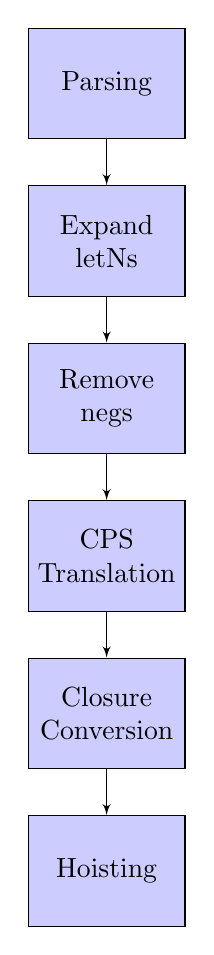
\begin{tikzpicture}[node distance = 2cm, auto]
    % Place nodes
    \node[internalStage](parsing){Parsing};
    \node[internalStage, below of=parsing](expandLetNs){Expand letNs};
    \node[internalStage, below of=expandLetNs](removeNegs){Remove negs};
    \node[internalStage, below of=removeNegs](cpsTrans){CPS Translation};
    \node[internalStage, below of=cpsTrans](clConv){Closure Conversion};
    \node[internalStage, below of=clConv](hoisting){Hoisting};

    
    \path[conversion] (parsing) -- (expandLetNs);
    \path[conversion] (expandLetNs) -- (removeNegs);
    \path[conversion] (removeNegs) -- (cpsTrans);
    \path[conversion] (cpsTrans) -- (clConv);
    \path[conversion] (clConv) -- (hoisting);

%    \node [block] (init) {initialize model};
%    \node [cloud, left of=init] (expert) {expert};
%    \node [cloud, right of=init] (system) {system};
%    \node [block, below of=init] (identify) {identify candidate models};
%    \node [block, below of=identify] (evaluate) {evaluate candidate models};
%    \node [block, left of=evaluate, node distance=3cm] (update) {update model};
%    \node [decision, below of=evaluate] (decide) {is best candidate better?};
%    \node [block, below of=decide, node distance=3cm] (stop) {stop};
%    % Draw edges
%    \path [line] (init) -- (identify);
%    \path [line] (identify) -- (evaluate);
%    \path [line] (evaluate) -- (decide);
%    \path [line] (decide) -| node [near start] {yes} (update);
%    \path [line] (update) |- (identify);
%    \path [line] (decide) -- node {no}(stop);
%    \path [line,dashed] (expert) -- (init);
%    \path [line,dashed] (system) -- (init);
%    \path [line,dashed] (system) |- (evaluate);
\end{tikzpicture}

% based on from system F...
\subsection{Parsing}
\subsection{CPS-Translation}

% y = var, i = int, f = fresh idn
\begin{figure}[ht]
\begin{alignat*}{2}
&\cpstrans{y} k &&\eqdef k(y) \\
%
&\cpstrans{i} k &&\eqdef k(i) \\
%
&\cpstrans{(\text{if}\ e_1\ e_2\ e_3)} k &&\eqdef \cpstrans{e_1} (\lambda x.(\text{if}\ x\ \cpstrans{e_2}k\ \cpstrans{e_3}k))) \\
%
&\cpstrans{(\text{lambda}\ (p_1, \dots, p_n)\ e)} k &&\eqdef k((\text{lambda}\ (cont, p_1, \dots, p_n)\ \\
&&&\hspace{1cm}\cpstrans{e}cont)) \\
%
&\cpstrans{(\text{define}\ (name, p_1, \dots, p_n)\ e)} k &&\eqdef k((\text{define}\ (name, cont, p_1, \dots, p_n)\ \\
&&&\hspace{1cm}\cpstrans{e}cont)) \\
%
&\cpstrans{(proc\ p_1, \dots, p_n)} k &&\eqdef \cpstrans{proc} \lambda x_{proc}.\cpstrans{p_1} \lambda x_1. \dots \\
&&&\hspace{1cm}\cpstrans{p_n} \lambda x_n.\\
&&&\hspace{1.5cm}(x_{proc}\ \lambda x_k.k(x_k), x_1, \dots, x_n) \\
%
&\cpstrans{(prim\ p_1, \dots, p_n)} k &&\eqdef \cpstrans{p_1} \lambda x_1. \dots  \\
&&&\hspace{1 cm}\cpstrans{p_n} \lambda x_n.\\
&&&\hspace{1.5 cm}(prim\ \lambda x_k.k(x_k), x_1, \dots, x_n) \\
%
&\cpstrans{(\text{let}\ ((idn\ e_1))\ e_2)} k &&\eqdef \cpstrans{e_1} \lambda x_1. \\
&&&\hspace{1 cm}(\text{let}\ idn = x_1\ \text{in}\ \cpstrans{e_2} \lambda x_2.(k(x_2)))\\
\end{alignat*}
\caption{CPS translation}
\end{figure}

This stage converts the program to continuation-passing style (CPS). Because it is the central stage of the compilation pipeline, we will first explain continuation-passing style in general before describing the particularities of the CPS-translation in the LJSP compiler.

\subsubsection{Continuation-Passing Style}

\subsubsection{CPS-Translation in LJSP}
\cite{sysftal}


\subsection{Closure Conversion}
\subsection{Hoisting}
\subsection{Conversion to asm.js}
\subsection{Code emission}

\chapter{Implementation}
\section{Scala}
\section{Problems encountered \& resolved}
% variables that contain functions, ftables generated at compile time
\section{Experimentation \& Optimisation}
% array index vars of type int, others of type double
% (array index vars are all generated, user doesn't see them)

\chapter{Testing}
This chapter describes the methods that were used to test the different subsystems of the LJSP compiler. While testing is imperative for all software development projects, it is especially important in compiler development. The reason for this is that it is usually impossible to determine whether or not the result given by the compiler is correct simply by looking at the generated code. \\

During the development of LJSP, two means of testing were being used:
\begin{itemize}
\item A custom testing framework written in Python that covers all of the frontend stages and some of the backend stages.
\item A ray tracer written in JavaScript that was used to test generated asm.js code specifically.
\end{itemize}
The following two sections will describe both systems in detail.

\section{Testing using \texttt{run_tests.py}}
Early on in the development of LJSP, it became necessary to test the output of every front end stage 
\section{Testing using the ray tracer}
% because asm.js evaluates to the same result regardless of
% whether or not it's compiled according to asm.js specification,
% it's possible to add invalid statements and still test the module

% ray tracer to test performance

\chapter{Evaluation}
% ast transformations would be nicer if the compiler generated the subtrees
% from short code snippets instead of creating the objects manually
\section{Evaluation against requirements}
\section{Strengths \& Weaknesses}

\chapter{Professional Issues}
% http://www.bcs.org/category/6030

\chapter{Conclusions}
\section{Future Work}
\subsection{Optimisations}
\subsection{Types}

\chapter{Bibliography}
\begin{thebibliography}{1}
  \bibitem{sysftal} Morrisett, Greg and Walker, David and Crary, Karl and Glew, Neal (1999). {\em From System F to Typed Assembly Language}, ACM Trans. Program. Lang. Syst.

\end{thebibliography}
\begin{appendices}

\chapter{User Guide}
\section{Compiler}
\section{Ray Tracer}
\section{Testing}

\chapter{Class diagrams}

\chapter{Programs Listings}

\end{appendices}

\end{document}
